\chapter{Schall, Quantenoszillatoren und der zweite Hauptsatz}

\lectureoverview{Der zweite Hauptsatz ist das Ziel, doch zwei konkrete Rechnungen bereiten den Weg. Die Schallgeschwindigkeit zeigt, wie thermodynamische Ableitungen zu beobachtbarer Bewegung führen. Der harmonische Oszillator macht anschließend das Versagen der klassischen Gleichverteilung bei steifen Freiheitsgraden deutlich und zeigt, wie die Quantenmechanik Moden nach und nach aktiviert. Schließlich kehren wir zum scheinbaren Widerspruch zwischen reversibler mikroskopischer Dynamik und zunehmender Entropie zurück. Mithilfe des Phasenraumflusses, der Grobkörnung, des Chaos und der Wiederkehr formulieren wir den zweiten Hauptsatz als ein überwältigend wahrscheinliches Gesetz statt als ausnahmsloses mechanisches Verbot.}

\section{Ein Versprechen zum zweiten Hauptsatz}

Das zentrale Problem lässt sich leicht formulieren, aber nur schwer erklären. Newtonsche Gleichungen sind reversibel: Ist ein mikroskopischer Verlauf erlaubt, so ist auch der zeitlich umgekehrte Verlauf erlaubt. Der zweite Hauptsatz besagt dennoch, dass makroskopische Prozesse eine bevorzugte Richtung haben, die dadurch gekennzeichnet ist, dass die Entropie gewöhnlich zunimmt. Auf diesen Widerspruch kommen wir zurück, aber nicht sofort. Zunächst ist es besser zu sehen, wie die statistische Mechanik konkrete Ergebnisse liefert; anschließend begegnen wir in einer elementaren Rechnung dem historischen Rätsel, das die klassische Physik zum Übergang zur Quantenphysik zwang.

Das erste Beispiel ist eine numerische, bewusst grobe Abschätzung: Wir schätzen die Schallgeschwindigkeit in einem verdünnten Gas. Das zweite ist innerhalb seiner Annahmen exakt: Wir berechnen die mittlere Energie eines harmonischen Oszillators in einem Wärmebad. Der Oszillator führt von der Gleichverteilung zu quantisierten Energieniveaus, von einer Mode zu unendlich vielen Moden und schließlich zurück zur Frage, was es bedeutet, dass ein Vielteilchensystem seinen Anfangszustand vergisst.

\section{Die molekulare Größenordnung der Schallgeschwindigkeit}

Betrachten wir eine kleine Überdichte in einem verdünnten Gas. Sie breitet sich aus, weil Moleküle den dicht besetzten Bereich verlassen; ihre Ausbreitungsgeschwindigkeit sollte daher mit der Molekülgeschwindigkeit vergleichbar sein. Aus der Gleichverteilung folgt die kinetische Energie eines Moleküls:
\begin{equation}
 \frac{3}{2}k_B T
 =\frac{1}{2}m\expect{v^2},
 \qquad
 \expect{v^2}=\frac{3k_B T}{m}.
 \label{eq:sm7-molecular-speed}
\end{equation}
Hier wird die Temperatur vom absoluten Nullpunkt aus gemessen, und \(k_B\) ist wieder eingesetzt, weil wir Laboreinheiten verwenden wollen. Das Argument liefert lediglich eine Größenordnung: Die quadratische Mittelgeschwindigkeit der Moleküle ist nicht selbst die Geschwindigkeit einer kollektiven Schallwelle.

Eine systematischere Herleitung betrachtet ein kleines Gaselement. Ungleiche Drücke auf gegenüberliegenden Seiten üben eine resultierende Kraft aus; seine Beschleunigung ist umgekehrt proportional zur Massendichte. Das Ergebnis hat die Form
\begin{equation}
 c_s^2=
 \left(\frac{\partial P}{\partial \rho_m}\right)_{\cal C},
 \qquad
 \rho_m=m\rho,
 \label{eq:sm7-sound-general}
\end{equation}
wobei \(\rho\) die Teilchendichte ist und der Index \({\cal C}\) die thermodynamische Bedingung angibt, der die Störung folgt. In der Rechnung an der Tafel wird verwendet:
\begin{equation}
 P=\rho k_B T
 \quad\Longrightarrow\quad
 \frac{1}{m}
 \left(\frac{\partial P}{\partial\rho}\right)_T
 =\frac{k_B T}{m}.
 \label{eq:sm7-sound-isothermal}
\end{equation}
Dies ist die isotherme Abschätzung der Schallgeschwindigkeit. Sie unterscheidet sich von \eqref{eq:sm7-molecular-speed} beim Quadrat der Geschwindigkeit um den Faktor \(3\) und bei der Geschwindigkeit um \(\sqrt{3}\).

\begin{figure}[t]
\centering
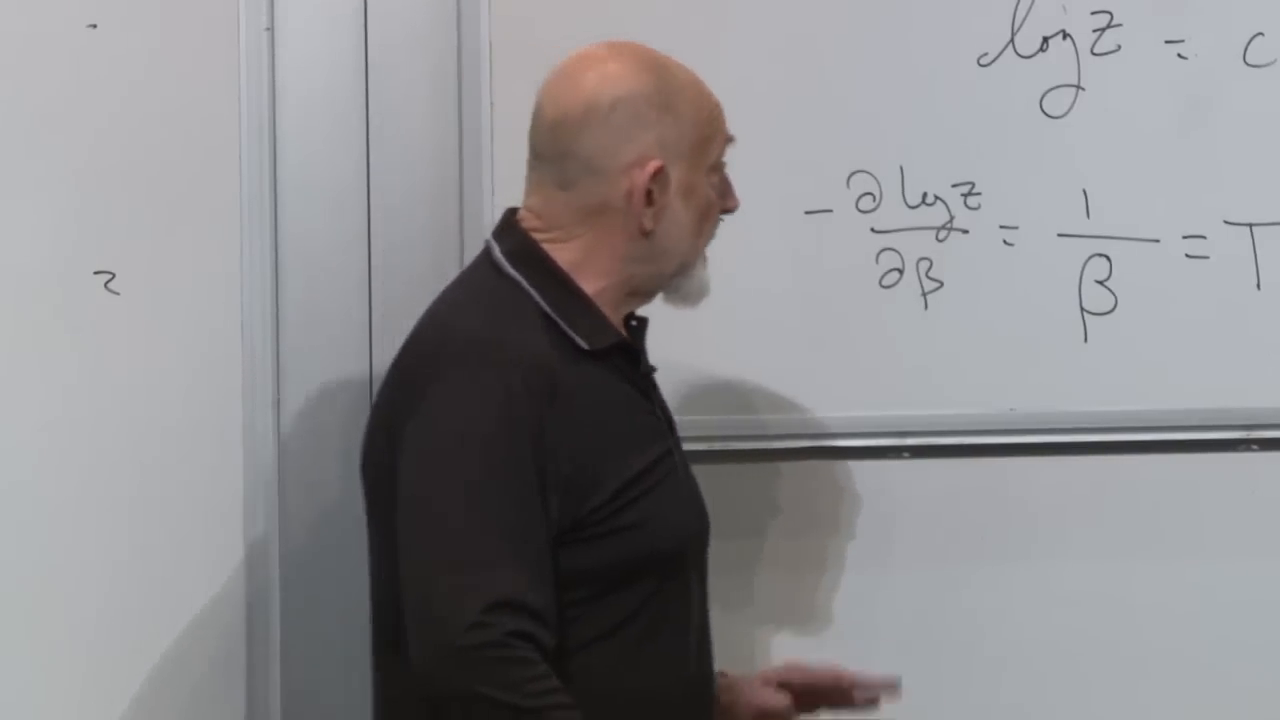
\includegraphics[width=0.90\textwidth]{lecture_07_figure_02.png}
\caption{Die Abschätzung der Molekülgeschwindigkeit, die Druckableitung und das eingesetzte ideale Gasgesetz nebeneinander.}
\lectureframe{00:08:55}
\end{figure}

Eine wichtige Präzisierung ist nötig. Eine Schallwelle kleiner Amplitude komprimiert und entspannt das Gas gewöhnlich schneller, als Wärme zwischen benachbarten Elementen fließen kann. Die lokale Bewegung ist daher näherungsweise adiabatisch, nicht isotherm:
\begin{equation}
 c_s^2=
 \left(\frac{\partial P}{\partial\rho_m}\right)_S.
 \label{eq:sm7-sound-adiabatic}
\end{equation}
Für ein ideales Gas mit dem Adiabatenexponenten \(\gamma\) gilt:
\begin{equation}
 P\rho_m^{-\gamma}=\text{constant},
 \qquad
 c_s^2=\gamma\frac{P}{\rho_m}
       =\gamma\frac{k_B T}{m}.
 \label{eq:sm7-sound-ideal-adiabatic}
\end{equation}
Für Luft bei Raumtemperatur ist \(\gamma\simeq 7/5\). Die Rechnung bei konstanter Temperatur liefert also eine brauchbare erste Abschätzung, während die adiabatische Ableitung die physikalisch angemessene Präzisierung darstellt.

Mit den groben Werten
\begin{equation}
\begin{aligned}
 k_B&\simeq1.3\times10^{-23}\ {\rm J\,K^{-1}},
 &T&\simeq300\ {\rm K},\\
 m_{\rm air}&\simeq4\times10^{-26}\ {\rm kg}.&&
\end{aligned}
 \label{eq:sm7-air-data}
\end{equation}
ergibt die Abschätzung anhand der Molekülgeschwindigkeit etwa \(500\ {\rm m\,s^{-1}}\). Die Temperatur muss hier als absolute Temperatur in Kelvin angegeben werden, nicht auf einer Skala mit einem willkürlichen Nullpunkt wie Fahrenheit. Die vertraute Schallgeschwindigkeit liegt in der Größenordnung von \(300\ {\rm m\,s^{-1}}\), und die adiabatische Formel für das ideale Gas ergibt bei Raumtemperatur etwa \(340\ {\rm m\,s^{-1}}\). Die grobe Rechnung hat somit die richtige physikalische Größenordnung getroffen.

\begin{figure}[t]
\centering
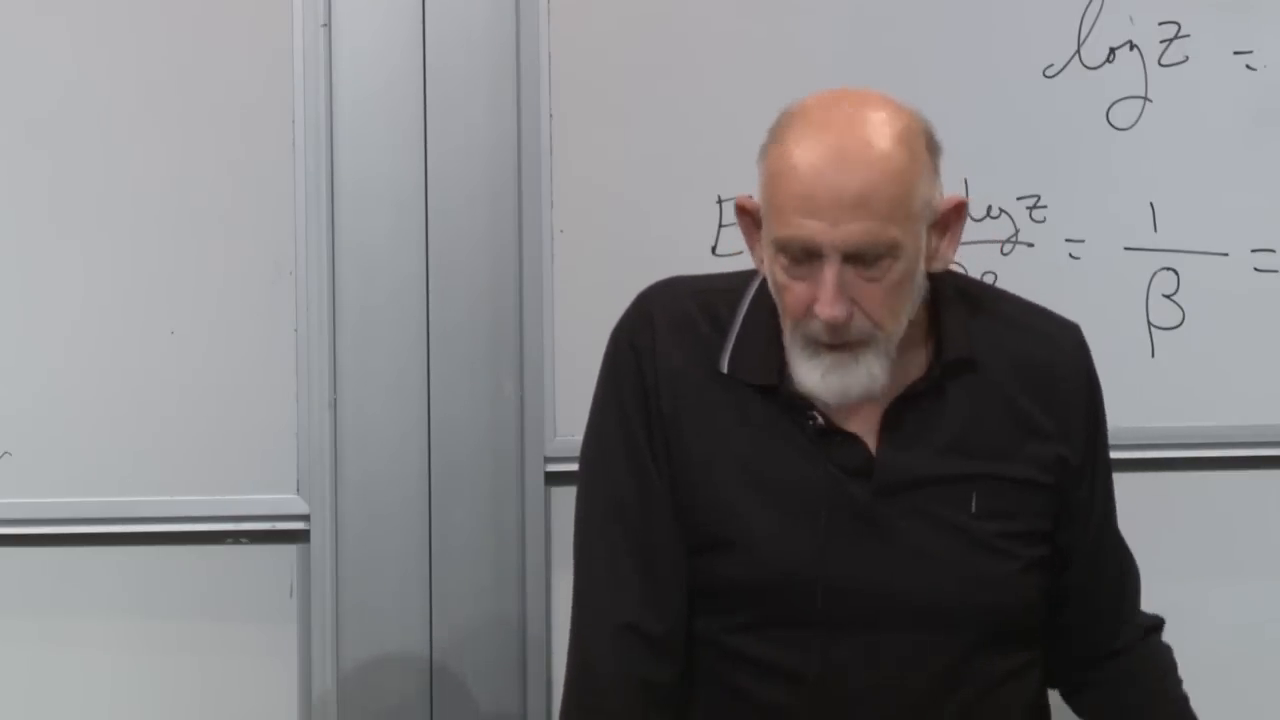
\includegraphics[width=0.90\textwidth]{lecture_07_figure_03.png}
\caption{Abschätzung für Luft bei Raumtemperatur mit der Boltzmann-Konstanten, einer effektiven Molekülmasse von ungefähr \(30\) Protonenmassen und \(T\simeq300\ {\rm K}\).}
\lectureframe{00:10:55}
\end{figure}

Lange bevor eine mikroskopische Erklärung verfügbar war, ließ sich die Schallgeschwindigkeit aus Messungen des Drucks als Funktion der Dichte bestimmen. Die statistische Herleitung liefert die bemerkenswerte Deutung, dass die resultierende makroskopische Geschwindigkeit durch die thermische Geschwindigkeit einzelner Moleküle festgelegt ist.

\begin{classroomqa}
\audiencequestion{Müssen Neutronen zur Molekülmasse hinzugerechnet werden, und zählt die Zahl \(14\) für Stickstoff nur Protonen?}
\lecturerresponse{Das angegebene Atomgewicht berücksichtigt bereits Protonen und Neutronen. Molekularer Stickstoff besteht aus zwei Atomen mit einem Atomgewicht von ungefähr \(14\); seine Masse beträgt also etwa \(28\) Protonenmassen. Für diese Abschätzung reicht es, \(28\) auf \(30\) zu runden.
\lecturetimestamp{00:10:58--00:11:16}}
\end{classroomqa}

\begin{classroomqa}
\audiencequestion{Der Faktor \(3\) stammt von den drei Translationsrichtungen, während sich der Schall in einer Richtung ausbreitet. Müsste der Faktor \(3\) deshalb wegfallen?}
\lecturerresponse{Das ist ein berechtigter Hinweis: Die dreidimensionale quadratische Mittelgeschwindigkeit der Moleküle darf nicht mit einer eindimensionalen Ausbreitungsgeschwindigkeit gleichgesetzt werden. Das einleitende Argument lieferte lediglich eine Größenordnung. Eine fundierte Antwort ergibt sich aus der Druckableitung zusammen mit der für die Welle passenden thermodynamischen Bedingung.
\lecturetimestamp{00:11:12--00:12:00}}
\end{classroomqa}

\begin{classroomqa}
\audiencequestion{Setzte die Ableitung voraus, dass die Temperatur während der Welle konstant bleibt?}
\lecturerresponse{Das Einsetzen des idealen Gasgesetzes in der gezeigten Rechnung tat dies. Für eine sehr kleine Störung ist eine Temperaturkonstanz eine plausible vorläufige Annahme. Die übliche Präzisierung lautet, dass gewöhnlicher Schall näherungsweise adiabatisch ist; dadurch wird die isotherme Ableitung durch \(\left(\partial P/\partial\rho_m\right)_S\) ersetzt.
\lecturetimestamp{00:12:59--00:14:01}}
\end{classroomqa}

\begin{classroomqa}
\audiencequestion{Wenn sowohl die Druck- als auch die Dichteänderungen klein sind, müsste dann nicht auch ihre Ableitung klein sein?}
\lecturerresponse{Nein. Eine Ableitung ist im infinitesimalen Grenzfall das Verhältnis zweier kleiner Änderungen. Sowohl \(\delta P\) als auch \(\delta\rho\) können klein sein, während \(\delta P/\delta\rho\) endlich bleibt und die Wellengeschwindigkeit festlegt.
\lecturetimestamp{00:14:03--00:14:23}}
\end{classroomqa}

\begin{classroomqa}
\audiencequestion{Müsste die Schallgeschwindigkeit steigen, wenn das Gas komprimiert wird, so wie sie beim Übergang vom Gas zur Flüssigkeit oder zum Festkörper steigt?}
\lecturerresponse{Ja. Die Ableitung wird am betrachteten Zustand ausgewertet, und \(P(\rho,T)\) muss nicht linear sein. Werden die Moleküle eng zusammengedrückt, wird die Zustandsgleichung nichtideal, und \(\partial P/\partial\rho\) kann erheblich anwachsen.
\lecturetimestamp{00:14:25--00:15:13}}
\end{classroomqa}

\begin{classroomqa}
\audiencequestion{Kann der Wert \(500\ {\rm m\,s^{-1}}\) bei jedem Druck verwendet werden?}
\lecturerresponse{Nein. Er gilt im Niederdichtebereich, in dem die ideale Gasgleichung eine gute Näherung ist. Sobald in \(P(\rho,T)\) höhere Dichtepotenzen auftreten, hängen die Ableitung und damit die Schallgeschwindigkeit von Druck und Dichte ab.
\lecturetimestamp{00:15:14--00:16:29}}
\end{classroomqa}

\begin{classroomqa}
\audiencequestion{Versagt auch das ursprüngliche Bild, nach dem sich der Schall ungefähr mit der Molekülgeschwindigkeit ausbreitet, wenn die Dichte zunimmt?}
\lecturerresponse{Wahrscheinlich. Dieses Bild ist auf ein verdünntes Gas zugeschnitten. Bei hoher Dichte gewinnen kollektive Wechselwirkungen zunehmend an Bedeutung. Genau deshalb ist die Ableitung der Zustandsgleichung die allgemeinere Beschreibung.
\lecturetimestamp{00:16:32--00:16:53}}
\end{classroomqa}

\begin{classroomqa}
\audiencequestion{Warum wurde die Masse eines Stickstoffmoleküls mit ungefähr \(30\) Protonenmassen angegeben und nicht mit \(28\)?}
\lecturerresponse{Es genügt die für die Abschätzung erforderliche numerische Genauigkeit; deshalb wurde \(28\) auf \(30\) gerundet. Teilt man die ursprüngliche Abschätzung von \(500\ {\rm m\,s^{-1}}\) durch \(\sqrt{3}\simeq1.7\), erhält man ebenfalls ungefähr \(300\ {\rm m\,s^{-1}}\). Die Korrektur lässt sich jedoch fundiert mit der adiabatischen Ableitung berechnen.
\lecturetimestamp{00:16:54--00:17:27}}
\end{classroomqa}

\section{Ein klassischer Oszillator in einem Wärmebad}

Nun ersetzen wir das frei bewegliche Molekül durch einen harmonischen Oszillator und behandeln alles Übrige als Wärmebad. Eine Masse an einer Feder ist das naheliegende Bild, doch das Modell ist viel allgemeiner. Eine elektromagnetische Hohlraummode schwingt; Atome in einem Kristall schwingen; fast jedes stabile System führt bei kleiner Auslenkung aus dem Gleichgewicht näherungsweise eine harmonische Bewegung aus.

Mit \(x\) als Auslenkung aus der Gleichgewichtslage, dem Impuls \(p\), der Masse \(m\) und der Federkonstanten \(\kappa\) lautet der Hamiltonoperator:
\begin{equation}
 H(x,p)=\frac{p^2}{2m}+\frac{\kappa x^2}{2},
 \qquad
 \omega=\sqrt{\frac{\kappa}{m}}.
 \label{eq:sm7-classical-hamiltonian}
\end{equation}
Das Wärmebad legt \(T\) fest, und von hier an verwenden wir wieder \(k_B=1\), sodass \(\beta=1/T\) gilt. Ein Oszillator, der mit einem Raum im Gleichgewicht ist, hat eine Temperatur nahe \(300\ {\rm K}\); in flüssigem Helium beträgt sie nur einige Kelvin. Eine gedachte Feder im Zentrum der Sonne würde nicht als Feder bestehen bleiben, doch das Beispiel verdeutlicht die Rolle der Umgebung. Der Boltzmann-Faktor zerfällt in ein Produkt:
\begin{equation}
 e^{-\beta H}
 =e^{-\beta p^2/(2m)}
  e^{-\beta\kappa x^2/2}.
 \label{eq:sm7-factorized-weight}
\end{equation}

\begin{figure}[t]
\centering
\includegraphics[width=0.90\textwidth]{lecture_07_figure_04.png}
\caption{Ein Feder-Masse-Oszillator und sein Hamiltonoperator als Summe aus kinetischer und potenzieller Energie.}
\lectureframe{00:20:55}
\end{figure}

Anders als beim freien Gas liefert das Ortsintegral nicht einfach das Volumen des Behälters. Das rücktreibende Potenzial gewichtet jede Auslenkung:
\begin{equation}
 Z_{\rm cl}
 =\frac{1}{h}\int_{-\infty}^{\infty}dp
             \int_{-\infty}^{\infty}dx\,
 e^{-\beta p^2/(2m)}
 e^{-\beta\kappa x^2/2}.
 \label{eq:sm7-classical-z}
\end{equation}
Der Faktor \(1/h\) macht die klassische Zustandssumme in einer Dimension dimensionslos. In der Rechnung an der Tafel wird er weggelassen, weil er unabhängig von \(\beta\) ist und die mittlere Energie nicht beeinflussen kann.

\begin{figure}[t]
\centering
\includegraphics[width=0.90\textwidth]{lecture_07_figure_05.png}
\caption{Die klassische Zustandssumme des Oszillators, zerlegt in die Gaußintegrale über Impuls und Auslenkung.}
\lectureframe{00:22:55}
\end{figure}

Für das Impulsintegral setzen wir
\begin{equation}
 q=\sqrt{\frac{\beta}{2m}}\,p,
 \qquad
 dp=\sqrt{\frac{2m}{\beta}}\,dq.
 \label{eq:sm7-p-gaussian-substitution}
\end{equation}
Für das Ortsintegral setzen wir
\begin{equation}
 y=\sqrt{\frac{\beta\kappa}{2}}\,x,
 \qquad
 dx=\sqrt{\frac{2}{\beta\kappa}}\,dy.
 \label{eq:sm7-x-gaussian-substitution}
\end{equation}
Da \(\int_{-\infty}^{\infty}e^{-u^2}\,du=\sqrt{\pi}\), lautet das unnormierte Phasenraumintegral aus der Rechnung an der Tafel:
\begin{equation}
 \int dp\,dx\,e^{-\beta H}
 =\frac{2\pi}{\beta}\sqrt{\frac{m}{\kappa}}
 =\frac{2\pi}{\beta\omega}.
 \label{eq:sm7-classical-z-unnormalized}
\end{equation}
Mit wieder eingesetzter Phasenraumzelle gilt:
\begin{equation}
 Z_{\rm cl}=\frac{2\pi}{h\beta\omega}
           =\frac{1}{\beta\hbar\omega}.
 \label{eq:sm7-classical-z-normalized}
\end{equation}

Für die Energie kommt es nur auf die Abhängigkeit von \(\beta\) an:
\begin{equation}
 \begin{aligned}
 \log Z_{\rm cl}&=\text{constant}-\log\beta,\\
 \expect{H}
 &=-\frac{\partial\log Z_{\rm cl}}{\partial\beta}\\
 &=\frac{1}{\beta}=T.
 \end{aligned}
 \label{eq:sm7-classical-energy}
\end{equation}

\begin{figure}[t]
\centering
\includegraphics[width=0.90\textwidth]{lecture_07_figure_06.png}
\caption{Die vollständige klassische Rechnung auf der rechten Tafel: Gaußfaktorzerlegung, \(Z\propto(\beta\omega)^{-1}\) und \(\expect{H}=1/\beta=T\).}
\lectureframe{00:30:15}
\end{figure}

Es gibt keinen Faktor \(3\), denn dies ist ein räumlicher Oszillator. Auch bleibt kein Faktor \(1/2\) übrig, denn es gibt zwei unabhängige quadratische Terme. Jeder Gaußterm liefert \(T/2\):
\begin{equation}
 \expect{K}=\frac{T}{2},
 \qquad
 \expect{U}=\frac{T}{2},
 \qquad
 \expect{H}=T.
 \label{eq:sm7-equipartition-oscillator}
\end{equation}
Dies ist die Gleichverteilung in ihrer nützlichsten Form: Jeder unabhängige quadratische Term im klassischen Hamiltonoperator trägt \(T/2\) bei.

Die Antwort ist unabhängig von \(m\) und \(\kappa\). Die Bewegung selbst hängt jedoch von diesen Parametern ab:
\begin{equation}
 \expect{p^2}=mT,
 \qquad
 \expect{x^2}=\frac{T}{\kappa},
 \qquad
 \expect{\dot{x}^2}=\frac{T}{m}.
 \label{eq:sm7-classical-fluctuations}
\end{equation}
Eine größere Masse bewegt sich also langsamer, und eine steifere Feder hat eine kleinere Amplitude, obwohl die mittlere Energie \(T\) bleibt. Beunruhigend wird das, wenn \(\kappa\) fantastisch groß wird. Eine Feder, die so steif ist, dass sie sich nicht bewegen kann, sollte wie eine starre Zwangsbedingung wirken; dennoch weist die klassische Gleichverteilung ihr weiterhin die Energie \(T\) zu.

\begin{classroomqa}
\audiencequestion{Wenn \(\kappa\to\infty\), geht die Zustandssumme gegen null. Wie kann ihr Logarithmus dann noch verwendet werden?}
\lecturerresponse{Wir halten \(\kappa\) endlich, aber beliebig groß. Sein Beitrag zu \(\log Z\) ist additiv und unabhängig von \(\beta\), sodass die \(\beta\)-Ableitung weiterhin \(T\) ergibt. Das Unbehagen im Grenzfall ist berechtigt: Die klassische Rechnung ist in sich konsistent, lässt aber eine Eigenschaft der Natur außer Acht, die bei sehr steifen Oszillatoren nötig ist.
\lecturetimestamp{00:34:01--00:34:54}}
\end{classroomqa}

\begin{classroomqa}
\audiencequestion{Für die Zustandssumme des idealen Gases war ein \(N!\) erforderlich. Müsste es hier einen entsprechenden Fakultätsfaktor geben?}
\lecturerresponse{Nein. Wir betrachten einen bestimmten Oszillator, keine Permutationen von \(N\) identischen Teilchen. Bei vielen unabhängigen, unterscheidbaren Moden multiplizieren sich die Zustandssummen. Ein Faktor zur Berücksichtigung der Ununterscheidbarkeit gehört zu einem anderen Zählproblem.
\lecturetimestamp{00:35:03--00:35:40}}
\end{classroomqa}

\section{Warum die klassische Gleichverteilung zur Krise führte}

Reale Moleküle sind keine strukturlosen Punkte. Ein zweiatomiges Molekül enthält eine schwingungsfähige Bindung und damit einen inneren Oszillator. Eine naive klassische Zählung würde dieser Mode selbst bei gewöhnlichen Temperaturen zusätzliche Wärmeenergie zuweisen. In einer bewusst schematischen Rechnung erhöht die Aktivierung eines Schwingungsoszillators die Energie von \(3T/2\) in Richtung \(5T/2\). Für eine genaue Wärmekapazitätsrechnung müssen auch Rotationsfreiheitsgrade berücksichtigt und Energie und ihre Temperaturableitung unterschieden werden. Der entscheidende experimentelle Befund ist einfacher: Steife innere Moden trugen bei niedrigen Temperaturen nicht wie von der klassischen Gleichverteilung gefordert bei.

Man könnte leugnen, dass das Molekül eine innere Struktur hat, was absurd wäre, oder erkennen, dass der klassischen Mechanik eine Zutat fehlt. Diese Zutat ist die Quantenmechanik. Wir brauchen nur wenig davon: nämlich die Tatsache, dass ein harmonischer Oszillator äquidistante Energieniveaus hat.

\section{Der Quantenoszillator}

Zunächst verschieben wir den Energieursprung und schreiben das Anregungsspektrum als
\begin{equation}
 E_n^{\rm exc}=n\hbar\omega,
 \qquad n=0,1,2,\ldots.
 \label{eq:sm7-shifted-spectrum}
\end{equation}
Die Zustandssumme ist nun eine echte Summe statt eines Phasenraumintegrals:
\begin{align}
 Z_{\rm exc}
 &=\sum_{n=0}^{\infty}e^{-\beta n\hbar\omega} \notag\\
 &=1+x+x^2+\cdots
  =\frac{1}{1-x},
 \qquad x=e^{-\beta\hbar\omega}, \notag\\
 &=\frac{1}{1-e^{-\beta\hbar\omega}}.
 \label{eq:sm7-quantum-z}
\end{align}

\begin{figure}[t]
\centering
\includegraphics[width=0.90\textwidth]{lecture_07_figure_07.png}
\caption{Äquidistante Niveaus und Auswertung der geometrischen Reihe für die Zustandssumme des Quantenoszillators.}
\lectureframe{00:42:05}
\end{figure}

Durch Ableiten erhalten wir die mittlere Anregungsenergie:
\begin{align}
 E_{\rm exc}
 &=-\frac{\partial\log Z_{\rm exc}}{\partial\beta}
  =-\frac{1}{Z_{\rm exc}}
    \frac{\partial Z_{\rm exc}}{\partial\beta}
 \notag\\
 &=\hbar\omega\,
   \frac{e^{-\beta\hbar\omega}}
        {1-e^{-\beta\hbar\omega}}
  =\frac{\hbar\omega}{e^{\beta\hbar\omega}-1}.
 \label{eq:sm7-quantum-energy}
\end{align}

\begin{figure}[t]
\centering
\includegraphics[width=0.90\textwidth]{lecture_07_figure_08.png}
\caption{Die thermische Anregungsenergie, ermittelt aus der Ableitung der quantenmechanischen Zustandssumme nach \(\beta\).}
\lectureframe{00:46:05}
\end{figure}

\subsection{Hohe Temperaturen}

Wenn \(\beta\hbar\omega\ll1\), gilt:
\begin{equation}
 e^{-\beta\hbar\omega}
 =1-\beta\hbar\omega
  +O\!\left((\beta\hbar\omega)^2\right).
 \label{eq:sm7-high-t-expansion}
\end{equation}
Der Zähler von \eqref{eq:sm7-quantum-energy} nähert sich \(\hbar\omega\), während der Nenner in führender Ordnung \(\beta\hbar\omega\) ist. Daher gilt:
\begin{equation}
 E_{\rm exc}\simeq\frac{1}{\beta}=T.
 \label{eq:sm7-high-t-energy}
\end{equation}
Bei vielen Niveaudifferenzen innerhalb der thermischen Energie ergibt sich aus dem quantenmechanischen Ergebnis wieder die klassische Gleichverteilung.

\subsection{Niedrige Temperaturen}

Wenn \(\beta\hbar\omega\gg1\), ist die Exponentialfunktion sehr klein:
\begin{equation}
 E_{\rm exc}
 \simeq\hbar\omega e^{-\beta\hbar\omega}.
 \label{eq:sm7-low-t-energy}
\end{equation}
Die thermische Anregung des Oszillators ist exponentiell unterdrückt. In der verschobenen Konvention ist sie fast null; die physikalische Nullpunktsenergie wird weiter unten wieder eingesetzt.

\begin{figure}[t]
\centering
\includegraphics[width=0.90\textwidth]{lecture_07_figure_09.png}
\caption{Entwicklung bei niedriger Temperatur: Die erste thermische Anregung ist durch \(e^{-\beta\hbar\omega}\) unterdrückt.}
\lectureframe{00:51:55}
\end{figure}

Der Übergang findet statt, wenn
\begin{equation}
 \beta\hbar\omega\sim1,
 \qquad\text{or equivalently}\qquad
 T\sim\hbar\omega.
 \label{eq:sm7-crossover}
\end{equation}
Diese Bedingung hat eine direkte Bedeutung. Nach der klassischen Gleichverteilung hätte der Oszillator die Energie \(T\). Quanteneffekte lassen sich nicht mehr vernachlässigen, wenn diese Energieskala unter eine Niveaudifferenz sinkt. Somit gilt:
\begin{equation}
\begin{aligned}
 \hbar\omega\gg T&:\quad \text{frozen and quantum},\\
 \hbar\omega\ll T&:\quad \text{active and classical}.
\end{aligned}
 \label{eq:sm7-regimes}
\end{equation}
Eine steifere Feder hat ein größeres \(\omega=\sqrt{\kappa/m}\) und benötigt daher eine höhere Temperatur, bevor sie sich klassisch verhält.

\section{Mit steigender Temperatur werden Freiheitsgrade sichtbar}

Bei niedriger Temperatur kann ein zweiatomiges Molekül thermisch einem Punktteilchen ähneln, weil seine steife Bindungsschwingung eingefroren ist. Wenn \(T\) \(\hbar\omega\) durchläuft, wird die Schwingungsmode aktiviert. Rotationsmoden können sich schon bei einer niedrigeren Temperaturskala aktivieren; noch höhere Temperaturen machen weitere innere Bewegungen sichtbar und ionisieren schließlich das Atom. Beim Erwärmen wird nicht einfach mehr Energie in eine feste Liste von Moden eingebracht. Es werden Freiheitsgrade sichtbar, die bei niedrigeren Temperaturen unsichtbar waren.

Ein gedachtes verschachteltes Molekül verdeutlicht den Punkt. Zwei Atome sind durch eine steife Feder verbunden; eines der scheinbaren Atome ist selbst ein Paar, das durch eine noch steifere Feder verbunden ist. Bei niedriger Temperatur \(T\) erscheinen beide Strukturen punktförmig. Bei der ersten Schwelle tritt die äußere Schwingung hervor, bei der zweiten wird die innere Struktur sichtbar. Die Komplexität des Systems erschließt sich eine Energieskala nach der anderen.

\begin{classroomqa}
\audiencequestion{Wenn ein Oszillator bereits im klassischen Bereich ist, wird die Feder dann durch weiteres Erwärmen steifer oder ändert sich ihre Frequenz?}
\lecturerresponse{Nein. Federkonstante und Frequenz bleiben unverändert. Eine höhere Temperatur führt zu größeren typischen Impulsen und Amplituden und damit zu größerer Energie. Die Steifigkeit bestimmt die Temperatur, bei der das klassische Gesetz einsetzt, nicht eine temperaturabhängige Versteifung der Feder.
\lecturetimestamp{01:03:17--01:05:11}}
\end{classroomqa}

\subsection{Kristalle und Einsteins spezifische Wärme}

Ein Kristall enthält sehr viele Schwingungsmoden. Die klassische Gleichverteilung weist jedem aktiven Oszillator eine Energie in der Größenordnung von \(T\) zu und überschätzt daher die Wärmekapazität bei niedrigen Temperaturen. Einsteins 1907-Modell behandelte Kristallschwingungen quantenmechanisch und erklärte, warum sie unterdrückt sind, bis die thermische Energie ihre Niveaudifferenz erreicht. Genauere Festkörpermodelle berücksichtigen eine Verteilung der Modenfrequenzen; das Prinzip des Ausfrierens ist jedoch bereits in Einsteins Rechnung enthalten.

\begin{classroomqa}
\audiencequestion{War dies die Arbeit, für die Einstein den Nobelpreis erhielt, und entstand sie erst, nachdem sich die Quantenmechanik etabliert hatte?}
\lecturerresponse{Nein. Die Nobelpreisbegründung bezog sich auf den photoelektrischen Effekt. Das Modell der spezifischen Wärme wurde 1907 veröffentlicht, lange bevor die Grundlagen der Quantenmechanik vollständig verstanden waren. Einstein griff entscheidende Quantenideen auf und entwickelte sie weiter, obwohl er später Aspekten der ausgereiften Theorie widersprach.
\lecturetimestamp{00:58:38--01:03:16}}
\end{classroomqa}

\begin{classroomqa}
\audiencequestion{Die klassische statistische Mechanik ersetzte eine Summe über diskrete Zustände durch ein scheinbar gleichförmiges Integral über Ort und Impuls. Was rechtfertigt diese Zustandszählung?}
\lecturerresponse{Die letztliche Rechtfertigung ergibt sich aus der Quantenmechanik. Im Hochtemperaturgrenzfall,
\[
 Z_{\rm exc}\simeq\frac{1}{\beta\hbar\omega},
\]
was genau mit dem dimensionslosen klassischen Ergebnis \eqref{eq:sm7-classical-z-normalized} übereinstimmt. Wenn die Abstände zwischen den Energieniveaus nicht aufgelöst werden, gehen die quantenmechanischen Zellen im Phasenraum in das klassische Phasenraummaß über.
\lecturetimestamp{00:59:38--01:03:06}}
\end{classroomqa}

\subsection{Eine Saite enthält unendlich viele Oszillatoren}

Eine Violin- oder Gitarrensaite lässt sich in Normalmoden zerlegen: die Grundschwingung, höhere Harmonische und immer kürzere Wellenlängen. Mathematisch gibt es unendlich viele Oszillatormoden. Würde die klassische Gleichverteilung jeder davon die Energie \(T\) zuweisen, hätte die Saite im thermischen Gleichgewicht unendliche Energie. Die Quantenmechanik verhindert diese Katastrophe. Die Moden mit den kürzesten Wellenlängen haben die höchsten Frequenzen und bleiben bei jeder endlichen Temperatur eingefroren; mit zunehmendem \(T\) werden nach und nach mehr Moden aktiviert. Dieselbe Überlegung wird später der Schwarzkörperstrahlung zugrunde liegen.

\begin{figure}[t]
\centering
\includegraphics[width=0.90\textwidth]{lecture_07_figure_10.png}
\caption{Mehrere überlagerte Normalmoden einer Saite veranschaulichen, warum eine kontinuierliche Saite eine unendliche Menge harmonischer Oszillatoren darstellt.}
\lectureframe{01:09:30}
\end{figure}

\begin{classroomqa}
\audiencequestion{Lässt sich der Übergang von der Quanten- zur klassischen Beschreibung direkt beobachten, und kann Erwärmung das Tieftemperaturverhalten umkehren?}
\lecturerresponse{Ja. Die Temperaturabhängigkeit der spezifischen Wärme eines Kristalls macht das Ausfrieren und die anschließende Aktivierung von Schwingungsmoden klar messbar.
\lecturetimestamp{01:09:11--01:10:13}}
\end{classroomqa}

\begin{classroomqa}
\audiencequestion{Wiederholt man bei vielen Oszillatoren für jede Mode die Zustandssumme eines einzelnen Oszillators?}
\lecturerresponse{Für unabhängige Moden gilt
\[
\begin{aligned}
 Z_{\rm tot}&=\prod_j Z_j,&
 \log Z_{\rm tot}&=\sum_j\log Z_j,\\
 E_{\rm tot}&=\sum_j E_j.&&
\end{aligned}
\]
Moden mit \(\hbar\omega_j\gg T\) leisten einen exponentiell kleinen Beitrag zur Wärme; Moden unterhalb dieser Schwelle tragen merklich bei.
\lecturetimestamp{01:10:14--01:11:00}}
\end{classroomqa}

\begin{classroomqa}
\audiencequestion{Was ist aus der Nullpunktsenergie des Oszillators \(\hbar\omega/2\) geworden?}
\lecturerresponse{Die physikalischen Energieniveaus lauten
\[
 E_n=\left(n+\frac12\right)\hbar\omega.
\]
Folglich gilt
\[
 \begin{aligned}
 Z_{\rm phys}
 &=e^{-\beta\hbar\omega/2}Z_{\rm exc},\\
 E_{\rm phys}
 &=\frac{\hbar\omega}{2}
  +\frac{\hbar\omega}{e^{\beta\hbar\omega}-1}.
 \end{aligned}
\]
Der gemeinsame Energieversatz verändert weder die Besetzungswahrscheinlichkeiten der Niveaus noch die Entropie, die Wärmekapazität oder die thermische Anregungsenergie, verschiebt aber die absolute mittlere Energie um \(\hbar\omega/2\). Der Vorfaktor in \(Z\) hängt von \(\beta\) ab und darf daher nicht weggelassen werden, wenn die absolute Energie gesucht ist.
\lecturetimestamp{01:11:08--01:11:37}}
\end{classroomqa}

\section{Der zweite Hauptsatz als Rätsel der Reversibilität}

Nun können wir auf das angekündigte Problem zurückkommen. Der zweite Hauptsatz besagt, dass gewöhnliche makroskopische Entwicklung irreversibel ist und die Entropie tendenziell zunimmt. Die mikroskopische Hamiltonsche Entwicklung ist reversibel. Wie kann eine reversible Abbildung exakter Zustände ein irreversibles Gesetz für makroskopische Zustände hervorbringen?

Wir stellen das System durch einen Punkt in einem hochdimensionalen Phasenraum dar:
\[
 \Gamma=(q_1,\ldots,q_N,p_1,\ldots,p_N).
\]
Unser Wissen entspricht gewöhnlich keinem exakten Punkt. Nehmen wir an, es sei durch eine gleichförmige Wahrscheinlichkeitsdichte auf einem kompakten Gebiet \(A\) mit Volumen \(\Omega_A\) beschrieben:
\begin{equation}
 f(\Gamma)=
 \begin{cases}
  1/\Omega_A,&\Gamma\in A,\\
  0,&\Gamma\notin A.
 \end{cases}
 \label{eq:sm7-uniform-blob}
\end{equation}
In Einheiten mit \(k_B=1\) lautet die feinkörnige Gibbs-Entropie:
\begin{equation}
 S_{\rm fine}
 =-\int d\Gamma\,f\log f
 =\log\Omega_A.
 \label{eq:sm7-blob-entropy}
\end{equation}
Ein kleineres Gebiet bedeutet mehr Information und geringere Entropie. Damit ist das Vorzeichen festgelegt: Größere Ungewissheit vergrößert den besetzten Bereich und erhöht \(\log\Omega_A\).

\begin{figure}[t]
\centering
\includegraphics[width=0.90\textwidth]{lecture_07_figure_11.png}
\caption{Ein kompaktes Wahrscheinlichkeitsgebiet in einem schematischen zweidimensionalen Ausschnitt des vollständigen Orts-Impuls-Phasenraums.}
\lectureframe{01:20:20}
\end{figure}

\begin{classroomqa}
\audiencequestion{Ist das System physikalisch darauf beschränkt, innerhalb des eingezeichneten Bereichs zu bleiben, und befindet es sich bereits im Gleichgewicht?}
\lecturerresponse{Nein. Der Bereich beschreibt, was über den Anfangszustand bekannt ist, und ist keine Wand im Phasenraum. Der Anfangszustand muss keiner Gleichgewichtsverteilung entsprechen. Ein Gas, das anfangs in einem Tank in einer Zimmerecke eingeschlossen ist, liefert ein konkretes Beispiel für spezielle Information über einen Nichtgleichgewichtszustand.
\lecturetimestamp{01:14:55--01:15:24}}
\end{classroomqa}

\section{Liouville-Fluss und Zunahme der grobkörnigen Entropie}

Das Theorem von Liouville besagt, dass der Hamiltonsche Fluss das Phasenraumvolumen erhält. Das exakte Gebiet kann sich verschieben, strecken, falten und extrem dünn werden, aber
\begin{equation}
 \Omega_{A(t)}=\Omega_{A(0)},
 \qquad
 S_{\rm fine}(t)=S_{\rm fine}(0).
 \label{eq:sm7-liouville}
\end{equation}
Das diskrete Analogon ist eine reversible Permutation von Zuständen. Weiß man anfangs, dass ein Würfel in einem von zwei Zuständen ist, kann eine bijektive Entwicklung diese beiden Zustände verändern, nicht aber die Anzahl der Möglichkeiten.

Reale Beschreibungen haben eine endliche Auflösung. Die Quantenmechanik liefert eine natürliche Phasenraumzelle; auch ein klassisches Experiment hat eine endliche Messgenauigkeit, selbst wenn man die Quantentheorie nicht heranzieht. Unter Hamiltonschem Fluss kann das Gebiet zu einer langen, dünnen Schlange werden. Sinkt der Abstand zwischen benachbarten Windungen unter die Auflösungsskala, fassen wir jede nicht aufgelöste Umgebung zu einer grobkörnigen Zelle zusammen. Das exakt besetzte Volumen bleibt konstant, doch die Vereinigung der grobkörnigen Zellen wächst:
\begin{equation}
 \Omega_{\rm coarse}(t)\geq\Omega_{A(t)},
 \qquad
 S_{\rm coarse}(t)=\log\Omega_{\rm coarse}(t).
 \label{eq:sm7-coarse-entropy}
\end{equation}

\begin{figure}[t]
\centering
\includegraphics[width=0.90\textwidth]{lecture_07_figure_12.png}
\caption{Ein volumenbewahrendes Filament, betrachtet mit endlichen Auflösungszellen. Das exakte schwarze Filament behält seine Fläche; die roten grobkörnigen Zellen nehmen einen größeren effektiven Bereich ein.}
\lectureframe{01:22:10}
\end{figure}

\begin{classroomqa}
\audiencequestion{Die grob aufgelösten Zellen überlappen. Verletzt das den Satz von Liouville?}
\lecturerresponse{Nein. Die Liouville-Dynamik betrifft die exakte Faser, die eineindeutig bleibt und das Volumen erhält. Die Überlappung entsteht in unserer unscharfen Beschreibung: Wir haben die Information darüber verworfen, in welchem dünnen Strang sich der Zustand befindet.
\lecturetimestamp{01:21:32--01:21:50}}
\end{classroomqa}

Ein nützlicher Vergleich ist Baumwolle. Das Materialvolumen aller Fasern kann nahezu gleich bleiben, während ein auseinandergezupfter Knäuel für einen Beobachter, der die einzelnen Fasern nicht auflösen kann, ein großes scheinbares Volumen einnimmt. Ebenso bildet ein Phasenraumgebiet immer feinere Tentakel aus; diese Tentakel entwickeln wiederum noch feinere Tentakel. Jede festgelegte endliche Auflösung reicht schließlich nicht mehr aus, um ihnen zu folgen.

\begin{classroomqa}
\audiencequestion{Scheint die Entropie klassisch nur zuzunehmen, während die Quantenmechanik diese Zunahme durch eine fundamentale Auflösungsgrenze real macht?}
\lecturerresponse{Für das Grobkörnig-Argument ist keine quantenmechanische Auflösungsgrenze erforderlich. Die Entropie bezieht sich sowohl auf das System als auch auf die makroskopischen Unterscheidungen, die in seiner Beschreibung erhalten bleiben. Bei unendlicher mikroskopischer Information bleibt die feinkörnige Entropie konstant; bei jeder festen endlichen Auflösung werden chaotische Fasern irgendwann unaufgelöst, und die grobkörnige Entropie nimmt zu.
\lecturetimestamp{01:24:04--01:25:20}}
\end{classroomqa}

\section{Chaos, ein endlicher zugänglicher Bereich und die Einstellung des Gleichgewichts}

Bei einem Gas in einem Kasten sind die Positionen beschränkt. Bei fester endlicher Gesamtenergie sind auch die Impulse beschränkt, selbst wenn sich die gesamte Energie vorübergehend in einem Teilchen konzentriert. Unter den üblichen Einschlussbedingungen hat die dynamisch zugängliche Energieschale daher ein endliches Maß.

\begin{figure}[t]
\centering
\includegraphics[width=0.90\textwidth]{lecture_07_figure_13.png}
\caption{Ein beschränkter zugänglicher Phasenraumbereich neben dem Filament und seiner grobkörnigen Darstellung.}
\lectureframe{01:28:10}
\end{figure}

Nahe beieinanderliegende Anfangspunkte in einem chaotischen System durchlaufen eine Zeit lang ähnliche Entwicklungen und entfernen sich dann voneinander. Bei einem Eröffnungsstoß beim Billard überträgt sich eine unmerkliche Änderung der Richtung des Spielballs auf die folgenden Kollisionen; die Unterschiede summieren sich, bis die Endkonfigurationen nichts mehr miteinander zu tun haben. Ein ganzes anfängliches Gebiet wird daher durch den zugänglichen Bereich gedehnt und gefaltet. Bei endlicher Auflösung nähert sich seine Beschreibung einem breiten, nahezu gleichförmigen Gleichgewichtszustand an.

\begin{figure}[t]
\centering
\includegraphics[width=0.90\textwidth]{lecture_07_figure_14.png}
\caption{Ein kompakter spezieller Zustand entwickelte sich im beschränkten zugänglichen Bereich zu einem komplizierten Filament, während sich die grob aufgelösten Zellen über eine viel größere Fläche verteilten.}
\lectureframe{01:33:10}
\end{figure}

Zwei Einschränkungen sind wichtig. Chaos allein beweist nicht, dass jede Trajektorie jede zugängliche Umgebung besucht; diese stärkere Aussage über das Abtasten des Phasenraums setzt eine ergodische oder mischende Eigenschaft voraus. Auch ist nicht jedes physikalische System chaotisch. Ein generisches Vielteilchengas und idealisierte Billards bilden den hier gemeinten Rahmen, in dem Mischen eine sinnvolle physikalische Erwartung ist.

\section{Rekurrenz hebt die Irreversibilität nicht auf}

Angenommen, alle Luftmoleküle befinden sich anfangs in einer Ecke und haben ein speziell vorbereitetes Geschwindigkeitsmuster. Durch Kollisionen verteilen sie sich rasch im Raum, und die grob aufgelöste Beschreibung erreicht das Gleichgewicht. In einem endlichen, maßtreuen Phasenraum besagt der Rekurrenzsatz von Poincaré, dass fast jeder Anfangspunkt beliebig nahe an seinen Ausgangspunkt zurückkehrt. Für eine Toleranz \(\epsilon>0\) ist eine Rekurrenzzeit \(t_R(\epsilon)\) unter den Voraussetzungen des Satzes endlich, auch wenn sie für ein makroskopisches System unvorstellbar groß ist. Eine exakte Rückkehr zu einem unendlich genau festgelegten Punkt ist weder erforderlich noch im Allgemeinen zu erwarten.

\begin{classroomqa}
\audiencequestion{Führt der Stoß auf den Spielball im Billardbeispiel Energie zu und macht er die abgeschlossene Entwicklung damit zunichte?}
\lecturerresponse{Der gewählte Anfangszustand beginnt unmittelbar nach dem Stoß; die dabei übertragene Energie ist also bereits berücksichtigt. Die Rekurrenz betrifft die anschließende isolierte, idealisierte Billarddynamik. Eine Rückkehr in die Nähe des Anfangszustands umfasst eine Konfiguration, in der sich der Spielball innerhalb der gewählten Toleranz dem Kugeldreieck nähert.
\lecturetimestamp{01:35:37--01:35:55}}
\end{classroomqa}

\begin{classroomqa}
\audiencequestion{Wenn das Gas schließlich in die Ecke zurückkehren kann, haben wir dann Information verloren, und ist das System wirklich reversibel?}
\lecturerresponse{Die mikroskopische Dynamik bleibt durchgehend reversibel. Die grob aufgelöste Entropie kann zunehmen, weil wir feine Korrelationen nicht mehr auflösen; dennoch kann eine außerordentlich seltene Fluktuation das System in die Nähe seines speziellen Anfangsmakrozustands zurückführen. Rekurrenz und grob aufgelöste Irreversibilität sind daher miteinander vereinbar.
\lecturetimestamp{01:37:34--01:38:15}}
\end{classroomqa}

Das führt zu Boltzmanns wesentlicher Formulierung. Die Entropie nimmt nicht in jedem logisch möglichen Augenblick zu. Für einen Nichtgleichgewichtsmakrozustand eines großen Systems führen überwältigend mehr der damit vereinbaren mikroskopischen Fortsetzungen zu größeren Makrozuständen als zu noch spezielleren. Die Entropie nimmt \emph{wahrscheinlich} zu. Abwärtsfluktuationen und Rekurrenzen sind möglich, doch ihre Wahrscheinlichkeiten und Zeitskalen machen sie in der gewöhnlichen makroskopischen Erfahrung unsichtbar. Das Irreversibilitätsproblem war eine der großen historischen Auseinandersetzungen der statistischen Mechanik und lastete schwer auf Boltzmann. Dieser historische Zusammenhang sollte nicht zu einer einfachen Kausalaussage über sein Leben gemacht werden.

\section{Was Chaos bedeutet}

Für eine stärker operationale Definition von Chaos nehmen wir an, dass sich zwei Anfangspunkte im Phasenraum um \(\delta\Gamma(0)\) unterscheiden. In einer chaotischen Richtung gilt typischerweise
\begin{equation}
 \lVert\delta\Gamma(t)\rVert
 \sim e^{\lambda t}\lVert\delta\Gamma(0)\rVert,
 \qquad \lambda>0,
 \label{eq:sm7-lyapunov-growth}
\end{equation}
in dem Bereich, in dem die linearisierte Separation aussagekräftig ist. Die Zahl \(\lambda\) ist ein Lyapunov-Exponent. Um Vorhersagen für eine Zeit \(t\) zu treffen, muss die Genauigkeit der Anfangsdaten ungefähr wie \(e^{-\lambda t}\) skaliert sein. Auch die Genauigkeit des dynamischen Gesetzes spielt eine Rolle: Modellfehler werden ebenso verstärkt wie Fehler der Anfangsbedingungen. Das Wetter ist das bekannte Beispiel.

\begin{classroomqa}
\audiencequestion{Gibt es ein Prinzip, dem zufolge \emph{die meisten} Systeme chaotisch sind, oder ist das lediglich eine empirische Feststellung?}
\lecturerresponse{Es gibt unendlich viele chaotische und nichtchaotische Hamiltonfunktionen; außerdem setzt schon das Wort \emph{die meisten} ein Maß auf dem Raum der Hamiltonfunktionen voraus. Komplizierte wechselwirkende Systeme sind oft chaotisch, aber es gibt keinen einfachen allgemeinen Test, mit dem sich jede Hamiltonfunktion durch bloße Inspektion klassifizieren lässt.
\lecturetimestamp{01:39:27--01:40:49}}
\end{classroomqa}

\begin{classroomqa}
\audiencequestion{Was bedeutet \emph{chaotisch} in dieser Diskussion genau?}
\lecturerresponse{Nahe beieinanderliegende Phasentrajektorien entfernen sich schnell genug voneinander, sodass langfristige Vorhersagen eine exponentiell genauere Kenntnis der Anfangsbedingungen erfordern. Im Gegensatz dazu drehen sich benachbarte Phasenraumpunkte beim harmonischen Oszillator gemeinsam und bleiben nahe beieinander. Auch das exakte Zweikörper-Keplerproblem ist nichtchaotisch, während das allgemeine Dreikörperproblem chaotische Bereiche aufweist.
\lecturetimestamp{01:40:50--01:43:45}}
\end{classroomqa}

\begin{classroomqa}
\audiencequestion{Müssen die Bewegungsgesetze ebenso genau bekannt sein wie die Anfangsbedingungen?}
\lecturerresponse{Ja. Beide Fehlerquellen pflanzen sich durch die Dynamik fort, und die chaotische Entwicklung verstärkt beide.
\lecturetimestamp{01:43:46--01:43:55}}
\end{classroomqa}

Das Doppelpendel ist ein anschauliches Beispiel. Ein gewöhnliches Pendel ist integrabel und vorhersagbar. Fügt man ein zweites Pendel hinzu, können Trajektorien, die fast am selben Ort beginnen, schließlich auf unterschiedliche Weise Energie übertragen und in völlig verschiedene Richtungen laufen.

\begin{figure}[t]
\centering
\includegraphics[width=0.90\textwidth]{lecture_07_figure_15.png}
\caption{Das Doppelpendel als konkretes Beispiel für deterministisches Chaos.}
\lectureframe{01:44:40}
\end{figure}

\begin{classroomqa}
\audiencequestion{Warum kann ein mechanisches System chaotisch sein, ein anderes aber nicht?}
\lecturerresponse{Das ist eine Eigenschaft der Hamiltonfunktion und ihrer invarianten Strukturen, keine Folge von Reibung oder experimentellem Rauschen. Sie zu bestimmen kann mathematisch schwierig sein; Komplexität ist ein Hinweis, aber kein Beweis.
\lecturetimestamp{01:44:03--01:45:58}}
\end{classroomqa}

\begin{classroomqa}
\audiencequestion{Ist ein ideales Doppelpendel auch ohne Reibung chaotisch?}
\lecturerresponse{Ja. Dissipation ist nicht erforderlich. Eine exakte deterministische Hamiltonsche Bewegung kann empfindlich von den Anfangsbedingungen abhängen. Unendlich genaue Anfangsdaten würden die Trajektorie auf unbegrenzte Zeit festlegen; bei endlicher Genauigkeit ist der Vorhersagehorizont jedoch endlich.
\lecturetimestamp{01:45:57--01:47:54}}
\end{classroomqa}

\begin{classroomqa}
\audiencequestion{Ist Chaos dasselbe wie das Fehlen einer geschlossenen Lösung?}
\lecturerresponse{Chaotischen Systemen fehlt im Allgemeinen eine global brauchbare geschlossene Darstellung der Trajektorie, aber analytische Lösbarkeit und empfindliche Abhängigkeit sind verschiedene Eigenschaften. Chaos wird dynamisch anhand der Trennung von Trajektorien diagnostiziert, nicht allein anhand unserer Unfähigkeit, eine Formel anzugeben.
\lecturetimestamp{01:48:20--01:49:23}}
\end{classroomqa}

\begin{classroomqa}
\audiencequestion{Worin unterscheidet sich allgegenwärtiges Chaos davon, genau auf dem instabilen Gipfel eines Hügels zu balancieren?}
\lecturerresponse{Der Hügelgipfel ist ein einzelner, außergewöhnlicher instabiler Zustand: Abseits davon müssen sich benachbarte Trajektorien nicht schnell voneinander entfernen. In einem chaotischen Gebiet ist die Instabilität entlang der Bahn typisch, und benachbarte Phasenraumpunkte entfernen sich wiederholt voneinander. Ein positiver Lyapunov-Exponent erfasst dieses anhaltende Wachstum.
\lecturetimestamp{01:49:27--01:50:11}}
\end{classroomqa}

\section{Von der mikroskopischen Bewegung zum statistischen Gesetz}

Die Abschätzung der Schallgeschwindigkeit zeigte, wie die mikroskopische thermische Bewegung eine makroskopische Ausbreitungsskala festlegt; die Fragen machten zugleich deutlich, welche thermodynamische Ableitung angegeben werden muss. Der Oszillator zeigte anschließend die Reichweite und das Versagen der klassischen Gleichverteilung. Die Quantisierung der Energieniveaus friert steife Moden ein, erklärt, warum sich Wärmekapazitäten mit der Temperatur ändern, und verhindert, dass unendlich viele hochfrequente Moden unendlich viel thermische Energie tragen.

Dieselbe Entwicklung von der exakten Mikrophysik zur effektiven makroskopischen Beschreibung löst den scheinbaren Widerspruch auf, der dem zweiten Hauptsatz zugrunde liegt. Die Hamiltonsche Strömung erhält das exakte Phasenraumvolumen und bleibt reversibel. Chaotisches Dehnen erzeugt feinere Korrelationen, als eine makroskopische Beschreibung erfasst; dadurch wächst der grob aufgelöste besetzte Bereich. Rekurrenz garantiert, dass seltene Rückkehrereignisse nicht ausgeschlossen sind; die Wahrscheinlichkeit erklärt, warum sie nicht zur gewöhnlichen Erfahrung gehören. Der zweite Hauptsatz ist keine neue irreversible mikroskopische Kraft. Er beschreibt die überwältigend zuverlässige statistische Entwicklungsrichtung für spezielle makroskopische Anfangsbedingungen in Systemen mit enorm vielen Freiheitsgraden.